%\subsection{Efficiency: Redundant Type Checks}

{  %% chapter slide
  \setbeamercolor{background canvas}{bg=sectioncolor}

\begin{frame}{\Challenge{5} Redundant Type Check}
  Select correct transition, avoiding \Emph{redundant type checks}.

  \medskip

  \scalebox{0.85}{\documentclass{standalone}
  \usepackage{tikz}
  \usetikzlibrary{arrows.meta, automata, bending, positioning, shapes.misc}
  \tikzstyle{automaton}=[shorten >=1pt, >={Stealth[bend,round]}, initial text=]

\begin{document}
\begin{tikzpicture}[automaton, auto, thick]
  \node[state,initial,rounded rectangle] (0) {$0$};
  \node[state,accepting,thick,rounded rectangle] (2) [right=30mm of 0] {$2$};
  \node[state,accepting,thick,rounded rectangle] (1) [above right=7mm and 30mm of 0] {$1$};
  \node[state,accepting,thick,rounded rectangle] (3) [below right=7mm and 30mm of 0] {$3$};
  \path[->] (0) edge node {$Int$} (2);
  \path[->] (0) edge[bend left=15]  node[pos=.8] {$Number~ \cap~ !Int$} (1);
  \path[->] (0) edge[bend right=15] node[swap] {$!~Number$} (3);
\end{tikzpicture}
\end{document}
}
\end{frame}
}


\newsavebox\typecaseAbox
\begin{lrbox}{\typecaseAbox}
  \begin{minipage}{8cm}
    %% dont re-indent this file
\begin{lstlisting}[style=reclojureClojure]
(typecase x
  (and Number (not Long))
  1

  Long
  2

  (not Number)
  3)
\end{lstlisting}

  \end{minipage}
\end{lrbox}

\newsavebox\typecaseITEbox
\begin{lrbox}{\typecaseITEbox}
  \begin{minipage}{8cm}
    %% dont re-indent this file
\begin{lstlisting}[style=reclojureScala]
Ite(N & !I, Some(1),
            Ite(I, Some(2),
                    Ite(!N, Some(3),
                           None)))
\end{lstlisting}

  \end{minipage}
\end{lrbox}

\newsavebox\typecaseITEafterbox
\begin{lrbox}{\typecaseITEafterbox}
  \begin{minipage}{8cm}
%% dont re-indent this file
\begin{lstlisting}[style=reclojureScala]
Ite(N, Ite(I, Some(2),
              Some(1)),
       Some(3))
\end{lstlisting}

  \end{minipage}
\end{lrbox}

\newsavebox\typecaseBabox
\begin{lrbox}{\typecaseBabox}
  \begin{minipage}{8cm}
%% dont re-indent this file
\begin{lstlisting}[style=reclojureScala]
if ~~N.typep(x)~~ {
  ... original code ...
} ~~ELSE~~ {
  ... original code ...
}
\end{lstlisting}

  \end{minipage}
\end{lrbox}

\newsavebox\typecaseBaabox
\begin{lrbox}{\typecaseBaabox}
  \begin{minipage}{8cm}
%% dont re-indent this file
\begin{lstlisting}[style=reclojureScala]
if ~~N.typep(x)~~ {
  if (N & !I).typep(x)
    Some(1)
  else if I.typep(x)
    Some(2)
  else if (!N).typep(x)
    Some(3)
  else      None
} ~~ELSE~~ {
  if (N & !I).typep(x)
    Some(1)
  else if I.typep(x)
    Some(2)
  else if (!N).typep(x)
    Some(3)
  else      None
}
\end{lstlisting}

  \end{minipage}
\end{lrbox}

\newsavebox\typecaseBbox
\begin{lrbox}{\typecaseBbox}
  \begin{minipage}{8cm}
    %% dont re-indent this file
\begin{lstlisting}[style=reclojureScala]
if N.typep(x) {
  if (N & !I).typep(x)
    Some(1)
  else if I.typep(x)
    Some(2)
  else if (!N).typep(x)
    Some(3)
  else      None
} else {
  if (N & !I).typep(x)
    Some(1)
  else if I.typep(x)
    Some(2)
  else if (!N).typep(x)
    Some(3)
  else      None
}
\end{lstlisting}

  \end{minipage}
\end{lrbox}

\newsavebox\typecaseCbox
\begin{lrbox}{\typecaseCbox}
  \begin{minipage}{6cm}
%% dont re-indent this file
\begin{lstlisting}[style=reclojureScala]
if N.typep(x) {
  if (STop & !I).typep(x)
    Some(1)
  else if I.typep(x)
    Some(2)
  else if (!STop).typep(x)
    Some(3)
  else      None
} else {
  if (SEmpty & !SEmpty).typep(x)
    Some(1)
  else if SEmpty.typep(x)
    Some(2)
  else if (!SEmpty).typep(x)
    Some(3)
  else None
}
\end{lstlisting}

  \end{minipage}
\end{lrbox}

\newsavebox\typecaseChbox
\begin{lrbox}{\typecaseChbox}
  \begin{minipage}{6cm}
%% dont re-indent this file
\begin{lstlisting}[style=reclojureScala]
if N.typep(x) {
  if (~~STop~~ & !I).typep(x)
    Some(1)
  else if I.typep(x)
    Some(2)
  else if (!~~STop~~).typep(x)
    Some(3)
  else      None
} else {
  if (~~SEmpty~~ & !~~SEmpty~~).typep(x)
    Some(1)
  else if ~~SEmpty~~.typep(x)
    Some(2)
  else if (!~~SEmpty~~).typep(x)
    Some(3)
  else None
}
\end{lstlisting}

  \end{minipage}
\end{lrbox}

\newsavebox\typecaseDbox
\begin{lrbox}{\typecaseDbox}
  \begin{minipage}{8cm}
    %% dont re-indent this file
\begin{lstlisting}[style=reclojureScala]
if N.typep(x) {
  if (!I).typep(x)
    Some(1)
  else if I.typep(x)
    Some(2)
  else if SEmpty.typep(x)
    Some(3)
  else None
} else {
  if SEmpty.typep(x)
    Some(1)
  else if SEmpty.typep(x)
    Some(2)
  else if STop.typep(x)
    Some(3)
  else None
}
\end{lstlisting}

  \end{minipage}
\end{lrbox}

\newsavebox\typecaseDhbox
\begin{lrbox}{\typecaseDhbox}
  \begin{minipage}{8cm}
    %% dont re-indent this file
\begin{lstlisting}[style=reclojureScala]
if N.typep(x) {
  if (~~!I~~).typep(x)
    Some(1)
  else if I.typep(x)
    Some(2)
  else if ~~SEmpty~~.typep(x)
    Some(3)
  else None
} else {
  if ~~SEmpty~~.typep(x)
    Some(1)
  else if SEmpty.typep(x)
    Some(2)
  else if ~~STop~~.typep(x)
    Some(3)
  else None
}
\end{lstlisting}

  \end{minipage}
\end{lrbox}

\newsavebox\typecaseEbox
\begin{lrbox}{\typecaseEbox}
  \begin{minipage}{8cm}
    %% dont re-indent this file
\begin{lstlisting}[style=reclojureScala]
if N.typep(x) {
  if (!I).typep(x)
    Some(1)
  else if I.typep(x)
    Some(2)
  else if false
    Some(3)
  else      None
} else {
  if false
    Some(1)
  else if false
    Some(2)
  else if true
    Some(3)
  else      None
}
\end{lstlisting}

  \end{minipage}
\end{lrbox}

\newsavebox\typecaseEhbox
\begin{lrbox}{\typecaseEhbox}
  \begin{minipage}{8cm}
    %% dont re-indent this file
\begin{lstlisting}[style=reclojureScala]
if N.typep(x) {
  if (!I).typep(x)
    Some(1)
  else if I.typep(x)
    Some(2)
  else if ~~FALSE~~
    Some(3)
  else      None
} else {
  if false
    Some(1)
  else if ~~FALSE~~
    Some(2)
  else if ~~TRUE~~
    Some(3)
  else      None
}
\end{lstlisting}

  \end{minipage}
\end{lrbox}

\newsavebox\typecaseFbox
\begin{lrbox}{\typecaseFbox}
  \begin{minipage}{8cm}
    %% dont re-indent this file
\begin{lstlisting}[style=reclojureScala]
if N.typep(x) {
  if (!I).typep(x)
    Some(1)
  else if I.typep(x)
    Some(2)
  else      None
} else Some(3)
\end{lstlisting}

  \end{minipage}
\end{lrbox}

\newsavebox\typecaseFhbox
\begin{lrbox}{\typecaseFhbox}
  \begin{minipage}{8cm}
    %% dont re-indent this file
\begin{lstlisting}[style=reclojureScala]
if N.typep(x) {
  if (!I).typep(x)
    Some(1)
  else if I.typep(x)
    Some(2)
  else ~~None~~
} else ~~Some(3)~~
\end{lstlisting}

  \end{minipage}
\end{lrbox}

\newsavebox\typecaseGabox
\begin{lrbox}{\typecaseGabox}
  \begin{minipage}{8cm}
%% dont re-indent this file
\begin{lstlisting}[style=reclojureScala]
if N.typep(x) {
  if ~~I.typep(x)~~ {
    ... original code...
  } ~~ELSE~~ {
    ... original code...
  }
} else Some(3)
\end{lstlisting}

  \end{minipage}
\end{lrbox}

\newsavebox\typecaseGbox
\begin{lrbox}{\typecaseGbox}
  \begin{minipage}{8cm}
    %% dont re-indent this file
\begin{lstlisting}[style=reclojureScala]
if N.typep(x) {
  if I.typep(x) {
    if (!I).typep(x)
      Some(1)
    else if I.typep(x)
      Some(2)
    else None
  } else {
    if (!I).typep(x)
      Some(1)
    else if I.typep(x)
      Some(2)
    else      None
  }
} else Some(3)
\end{lstlisting}

  \end{minipage}
\end{lrbox}

\newsavebox\typecaseGhbox
\begin{lrbox}{\typecaseGhbox}
  \begin{minipage}{8cm}
    %% dont re-indent this file
\begin{lstlisting}[style=reclojureScala]
if N.typep(x) {
  if ~~I.typep(x)~~ {
    if (!I).typep(x)
      Some(1)
    else if I.typep(x)
      Some(2)
    else None
  } ~~ELSE~~ {
    if (!I).typep(x)
      Some(1)
    else if I.typep(x)
      Some(2)
    else      None
  }
} else Some(3)
\end{lstlisting}

  \end{minipage}
\end{lrbox}


\newsavebox\typecaseHbox
\begin{lrbox}{\typecaseHbox}
  \begin{minipage}{8cm}
    %% dont re-indent this file
\begin{lstlisting}[style=reclojureScala]
if N.typep(x) {
  if I.typep(x) {
    if (!STop).typep(x)
      Some(1)
    else if STop.typep(x)
      Some(2)
    else None
  } else {
    if (!SEmpty).typep(x)
      Some(1)
    else if SEmpty.typep(x)
      Some(2)
    else None
  }
} else Some(3)
\end{lstlisting}

  \end{minipage}
\end{lrbox}

\newsavebox\typecaseHhbox
\begin{lrbox}{\typecaseHhbox}
  \begin{minipage}{8cm}
    %% dont re-indent this file
\begin{lstlisting}[style=reclojureScala]
if N.typep(x) {
  if I.typep(x) {
    if (!~~STop~~).typep(x)
      Some(1)
    else if ~~STop~~.typep(x)
      Some(2)
    else None
  } else {
    if (!~~SEmpty~~).typep(x)
      Some(1)
    else if ~~SEmpty~~.typep(x)
      Some(2)
    else None
  }
} else Some(3)
\end{lstlisting}

  \end{minipage}
\end{lrbox}

\newsavebox\typecaseIbox
\begin{lrbox}{\typecaseIbox}
  \begin{minipage}{8cm}
    %% dont re-indent this file
\begin{lstlisting}[style=reclojureScala]
if N.typep(x) {
  if I.typep(x) {
    if SEmpty.typep(x)
      Some(1)
    else if STop.typep(x)
      Some(2)
    else      None
  } else {
    if STop.typep(x)
      Some(1)
    else if SEmpty.typep(x)
      Some(2)
    else      None
  }
} else Some(3)
\end{lstlisting}

  \end{minipage}
\end{lrbox}

\newsavebox\typecaseIhbox
\begin{lrbox}{\typecaseIhbox}
  \begin{minipage}{8cm}
    %% dont re-indent this file
\begin{lstlisting}[style=reclojureScala]
if N.typep(x) {
  if I.typep(x) {
    if ~~SEmpty~~.typep(x)
      Some(1)
    else if STop.typep(x)
      Some(2)
    else      None
  } else {
    if ~~STop~~.typep(x)
      Some(1)
    else if SEmpty.typep(x)
      Some(2)
    else      None
  }
} else Some(3)
\end{lstlisting}

  \end{minipage}
\end{lrbox}

\newsavebox\typecaseJbox
\begin{lrbox}{\typecaseJbox}
  \begin{minipage}{8cm}
    %% dont re-indent this file
\begin{lstlisting}[style=reclojureScala]
if N.typep(x) {
  if I.typep(x) {
    if false
      Some(1)
    else if true
      Some(2)
    else      None
  } else {
    if true
      Some(1)
    else if false
      Some(2)
    else      None
  }
} else Some(3)
\end{lstlisting}

  \end{minipage}
\end{lrbox}

\newsavebox\typecaseJhbox
\begin{lrbox}{\typecaseJhbox}
  \begin{minipage}{8cm}
    %% dont re-indent this file
\begin{lstlisting}[style=reclojureScala]
if N.typep(x) {
  if I.typep(x) {
    if ~~FALSE~~
      Some(1)
    else if ~~TRUE~~
      Some(2)
    else      None
  } else {
    if true
      Some(1)
    else if ~~FALSE~~
      Some(2)
    else      None
  }
} else Some(3)
\end{lstlisting}

  \end{minipage}
\end{lrbox}

\newsavebox\typecaseKbox
\begin{lrbox}{\typecaseKbox}
  \begin{minipage}{8cm}
    %% dont re-indent this file
\begin{lstlisting}[style=reclojureClojure]
(if (typep x 'Integer)
    2
    (if (typep x 'Number)
        1
        3))
\end{lstlisting}

  \end{minipage}
\end{lrbox}


\newsavebox\typecaseKhbox
\begin{lrbox}{\typecaseKhbox}
  \begin{minipage}{8cm}
    %% dont re-indent this file
\begin{lstlisting}[style=reclojureScala]
if N.typep(x) {
  if I.typep(x)
    ~~Some(2)~~
  else
    ~~Some(1)~~
} else Some(3)
\end{lstlisting}

  \end{minipage}
\end{lrbox}



\begin{frame}[t]{Sequential Type Check}
  A DFA state may have several \Emph{disjoint} transitions.
  \begin{columns}
    \begin{column}{0.5\textwidth}
      \scalebox{0.9}{\documentclass{standalone}
  \usepackage{tikz}
  \usetikzlibrary{arrows.meta, automata, bending, positioning, shapes.misc}
  \tikzstyle{automaton}=[shorten >=1pt, >={Stealth[bend,round]}, initial text=]

\begin{document}
\begin{tikzpicture}[automaton, auto, thick]
  \node[state,initial,rounded rectangle] (0) {$0$};
  \node[state,accepting,thick,rounded rectangle] (2) [right=30mm of 0] {$2$};
  \node[state,accepting,thick,rounded rectangle] (1) [above right=7mm and 30mm of 0] {$1$};
  \node[state,accepting,thick,rounded rectangle] (3) [below right=7mm and 30mm of 0] {$3$};
  \path[->] (0) edge node {$Int$} (2);
  \path[->] (0) edge[bend left=15]  node[pos=.8] {$Number~ \cap~ !Int$} (1);
  \path[->] (0) edge[bend right=15] node[swap] {$!~Number$} (3);
\end{tikzpicture}
\end{document}
}
    \end{column}
    \begin{column}{0.5\textwidth}  %%
      \only<1>{\usebox\typecaseAbox}%
      \only<2>{\usebox\typecaseKbox}
    \end{column}
  \end{columns}

  \begin{itemize}
  \item<1->{Some types may be checked multiple times.}
  \item<2>{We can rewrite the code to \Emph{eliminate redundant checks}.}
  \end{itemize}

\end{frame}

\begin{frame}{Decision Tree Structure}
  We programmatically manipulate \code{if \code{\textcolor{greeny}{then}} ... \code{\textcolor{red}{else}} ...} using a decision tree.

  \begin{columns}
    \begin{column}{0.5\textwidth}
      \includegraphics[height=0.8\textheight]{ldd-0.pdf}
    \end{column}
    \begin{column}{0.5\textwidth}  %%
      \usebox\typecaseAbox
    \end{column}    
  \end{columns}
\end{frame}

\begin{frame}{Decision Tree, Before and After}
  Viewing the decision tree before/after

  \medskip
  
  Rewrite: $1 \to 2\to 3\to 4\to 5\to 6\to 7\to 8\to 9$

  \medskip
  
  \begin{columns}
    \begin{column}{0.5\textwidth}
      \includegraphics[height=0.8\textheight]{ldd-0.pdf}
    \end{column}
    \begin{column}{0.5\textwidth}  %%
      \includegraphics[height=0.8\textheight]{ldd-9.pdf}
    \end{column}
  \end{columns}
\end{frame}


%% Thanks to John Wickerson, https://tex.stackexchange.com/users/25356/john-wickerson
%% for this arrow
%% https://tex.stackexchange.com/questions/113228/how-can-i-add-a-big-arrow
\def\myLeftArrow{\smash{
  \begin{tikzpicture}[baseline=-2mm]
    \useasboundingbox (-2,0);
    \node[single arrow,draw=black,fill=red!10,minimum width=5cm,minimum height=7cm,shape border rotate=180] at (0,-1) {};
  \end{tikzpicture}
}}


\begin{frame}{Rewrite: $\colorbox{orange!30}{\Huge 1}\to 2\to 3\to 4\to 5\to 6\to 7\to 8\to 9$}%1
  Duplicate tree, and introduce \colorbox{pink!30}{\code{if (typep x N) \code{\textcolor{greeny}{then}} ... \code{\textcolor{red}{else}} ...}}

  \begin{columns}
    \begin{column}{0.5\textwidth}
      \only<1,2>{\includegraphics[height=0.8\textheight]{ldd-0.pdf}}%
    \end{column}
    \begin{column}{0.5\textwidth}  %%
      \only<2>{\includegraphics[height=0.8\textheight]{ldd-1.pdf}}%
    \end{column}    
  \end{columns}
\end{frame}

\begin{frame}{Rewrite: $\colorbox{orange!30}{\Huge 1}\to 2\to 3\to 4\to 5\to 6\to 7\to 8\to 9$}%1
  Duplicate tree, and introduce \colorbox{pink!30}{\code{if (typep x N) \code{\textcolor{greeny}{then}} ... \code{\textcolor{red}{else}} ...}}
  
  \centerline{  \includegraphics[height=0.8\textheight]{ldd-1.pdf}}
\end{frame}

\begin{frame}{Rewrite: $1\to \colorbox{orange!30}{\Huge 2}\to 3\to 4\to 5\to 6\to 7\to 8\to 9$}
\begin{tabular}{ll}
  In \code{\textcolor{greeny}{then}}: \colorbox{pink!30}{Supertypes of \code{N} $\to$ \code{:sigma}}. &
  In \code{\textcolor{red}{else}}: \colorbox{pink!30}{Subtypes of \code{N} $\to$ \code{:empty-set}}.
  \end{tabular}
  
  \only<1>{\centerline{\includegraphics[height=0.8\textheight]{ldd-1.pdf}}}%
  \only<2>{\centerline{\includegraphics[height=0.8\textheight]{ldd-2.pdf}}}
\end{frame}

\begin{frame}{Rewrite: $1\to 2\to \colorbox{orange!30}{\Huge 3}\to 4\to 5\to 6\to 7\to 8\to 9$}
  \begin{tabular}{ll}
    \colorbox{pink!30}{\code{(not :sigma)} $\to$ \code{:empty-set}} &       \colorbox{pink!30}{\code{(not :empty-set)} $\to$ \code{:sigma}}    
  \end{tabular}

  \only<1>{\centerline{\includegraphics[height=0.8\textheight]{ldd-2.pdf}}}%
  \only<2>{\centerline{\includegraphics[height=0.8\textheight]{ldd-3.pdf}}}
\end{frame}

\begin{frame}{Rewrite: $1\to 2\to 3\to \colorbox{orange!30}{\Huge 4}\to 5\to 6\to 7\to 8\to 9$}
  \begin{tabular}{ll}
    \colorbox{pink!30}{\code{(:sigma \& x)} $\to$ \code{x}} &       \colorbox{pink!30}{\code{(:empty-set \& x)} $\to$ \code{:empty-set}}
  \end{tabular}
  \only<1>{\centerline{\includegraphics[height=0.8\textheight]{ldd-3.pdf}}}%
  \only<2>{\centerline{\includegraphics[height=0.8\textheight]{ldd-4.pdf}}}
  
\end{frame}

\newsavebox\boxstop
\begin{lrbox}{\boxstop}
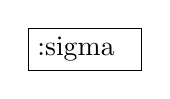
\begin{tikzpicture}
\node[draw,text width=1.2cm] at (2,-2) {\code{:sigma}};
\end{tikzpicture}
\end{lrbox}

\newsavebox\boxsempty
\begin{lrbox}{\boxsempty}
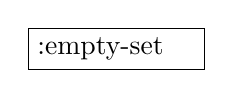
\begin{tikzpicture}
\node[draw,text width=2.0cm] at (2,-2) {\code{:empty-set}};
\end{tikzpicture}
\end{lrbox}


\begin{frame}{Rewrite: $1\to 2\to 3\to 4\to\colorbox{orange!30}{\Huge 5}\to 6\to 7\to 8\to 9$}
  \begin{tabular}{ll}
    Replace \usebox\boxstop~with \code{\textcolor{greeny}{then}} branch. &
    Replace \usebox\boxsempty~with \code{\textcolor{red}{else}} branch.
  \end{tabular}

  \only<1>{\centerline{\includegraphics[height=0.8\textheight]{ldd-4.pdf}}}%
  \only<2>{\centerline{\includegraphics[height=0.8\textheight]{ldd-5.pdf}}}
  
\end{frame}


\begin{frame}{Rewrite: $1\to 2\to 3\to 4\to 5\to \colorbox{orange!30}{\Huge 6}\to 7\to 8\to 9$}
  Duplicate tree, and introduce \colorbox{pink!30}{\code{if (typep x I) \code{\textcolor{greeny}{then}} ... \code{\textcolor{red}{else}} ...}}

  \begin{columns}
    \begin{column}{0.5\textwidth}
      \includegraphics[height=0.8\textheight]{ldd-5.pdf}%
    \end{column}

    \begin{column}{0.5\textwidth}  %%
      \includegraphics[height=0.8\textheight]{ldd-6.pdf}%
    \end{column}    
  \end{columns}
\end{frame}

\begin{frame}{Rewrite: $1\to 2\to 3\to 4\to 5\to \colorbox{orange!30}{\Huge 6}\to 7\to 8\to 9$}
  Duplicate tree, and introduce \colorbox{pink!30}{\code{if (typep x I) \code{\textcolor{greeny}{then}} ... \code{\textcolor{red}{else}} ...}}

  \centerline{\includegraphics[height=0.8\textheight]{ldd-6.pdf}}  %
\end{frame}


\begin{frame}{Rewrite: $1\to 2\to 3\to 4\to 5\to 6\to \colorbox{orange!30}{\Huge 7}\to 8\to 9$}
  \begin{tabular}{ll}
  In \code{\textcolor{greeny}{then}}: \colorbox{pink!30}{Supertypes of \code{I} $\to$ \code{:sigma}}.&
  In \code{\textcolor{red}{else}}: \colorbox{pink!30}{Subtypes of \code{I} $\to$ \code{:empty-set}}.
  \end{tabular}

  \only<1>{\centerline{\includegraphics[height=0.8\textheight]{ldd-6.pdf}}}%
  \only<2>{\centerline{\includegraphics[height=0.8\textheight]{ldd-7.pdf}}}
\end{frame}


\begin{frame}{Rewrite: $1\to 2\to 3\to 4\to 5\to 6\to 7\to \colorbox{orange!30}{\Huge 8}\to 9$}
  \begin{tabular}{ll}
      \colorbox{pink!30}{\code{(not :sigma)} $\to$ \code{:empty-set}} &    
      \colorbox{pink!30}{\code{(not :empty-set)} $\to$ \code{:sigma}}
  \end{tabular}

  \only<1>{\centerline{\includegraphics[height=0.8\textheight]{ldd-7.pdf}}}%
  \only<2>{\centerline{\includegraphics[height=0.8\textheight]{ldd-8.pdf}}}
\end{frame}

\begin{frame}{Rewrite: $1\to 2\to 3\to 4\to 5\to 6\to 7\to 8\to \colorbox{orange!30}{\Huge 9}$}
  \begin{tabular}{ll}
    Replace \usebox\boxstop~ with \code{\textcolor{greeny}{then}} branch. &
    Replace \usebox\boxsempty~ with \code{\textcolor{red}{else}} branch.
  \end{tabular}

  \only<1>{\centerline{\includegraphics[height=0.8\textheight]{ldd-8.pdf}}}%
  \only<2>{\centerline{\includegraphics[height=0.8\textheight]{ldd-9.pdf}}}
  

\end{frame}


\begin{frame}{Rewrite: Summary}
  Code has been rewritten so that \Emph{any type check occurs no more than once}.

  \begin{columns}
    \begin{column}{0.5\textwidth}
      \usebox\typecaseAbox
    \end{column}
    \begin{column}{0.5\textwidth}  %%
      \usebox\typecaseKbox
    \end{column}
  \end{columns}

  And it is clear the code never returns \code{nil}.

\end{frame}




